\chapter{Ecosystemen en trofische structuur}\label{ch:b1:ecosystem-organization}

Een bron in een kalksteenvlakte stort water uit dat zo helder is dat elke
plant, vis en schildpad erin vanuit een boot te tellen valt. Er valt
zonlicht op het zeegras met \qty{1.7}{} miljoen kilocalorieën per vierkante
meter per jaar; het gras slaat er één procent van op; de slakken en
schildpadden die het gras eten krijgen daarvan een zesde; de vissen die de
slakken eten opnieuw een tiende; en de ene reiger aan de top leeft van een
honderdduizendste van wat er op het water viel. Elk \omterm{def:b1:ecosystem-organization:ecosystem}{ecosysteem} is zo
gebouwd: een stroom energie die eenmaal binnenkomt, van eters naar
gegetenen gaat en als warmte vertrekt, terwijl de stof die zij verplaatst
wordt hergebruikt. Dit hoofdstuk omschrijft het \omterm{def:b1:ecosystem-organization:ecosystem}{ecosysteem} en zijn delen,
de \omterm{def:b1:ecosystem-organization:niche}{nis} die elke soort inneemt, de \omterm{def:b1:ecosystem-organization:trophic}{trofische niveaus} en voedselwebben
waardoorheen energie stroomt, de productiviteit die de omvang van het
geheel bepaalt, en de manieren om te tellen hoeveel soorten dingen erin
leven.

\section{Ecosysteem en nis}

\begin{definition}[Ecosysteem, biotoop, levensgemeenschap]\label{def:b1:ecosystem-organization:ecosystem}
\index{ecosysteem}\index{biotoop}\index{levensgemeenschap}
Een \emph{ecosysteem} is het geheel van de \omterm{def:b1:organism-environment:organism}{organismen} die op een bepaalde
plaats leven samen met de fysische omgeving die zij innemen en waarmee zij
uitwisselen: de \emph{levensgemeenschap} (of biocoenose) --- alle \omterm{def:b1:populations:population}{populaties}
van alle soorten --- en de \emph{biotoop} --- de bodem, het water, de lucht,
het licht en het klimaat. Zijn grenzen worden voor de vraag gekozen: een
rottende stam, een vijver, een bos, een oceaanbekken, de hele biosfeer. Een
ecosysteem is een \omterm{def:b1:organism-environment:organism}{open systeem} (\cref{ch:b1:organism-environment}): er
stroomt energie doorheen, er gaat stof in kringloop binnenin en over zijn
grenzen, en zijn structuur is het patroon van wie wie eet.
\end{definition}

\begin{definition}[Leefgebied, nis]\label{def:b1:ecosystem-organization:niche}
\index{ecologische nis}\index{leefgebied}
Het \emph{leefgebied} van een soort is waar zij leeft; haar \emph{nis} is
hoe zij leeft: het volledige stel omstandigheden dat zij verdraagt en
hulpbronnen dat zij gebruikt --- temperatuur, vocht, licht, voedsel, tijd
van activiteit, nestplaatsen --- elk daarvan een dimensie waarlangs de soort
een bereik inneemt. De \emph{fundamentele nis} is het bereik dat zij alleen
zou kunnen innemen; de \emph{gerealiseerde nis} het deel dat zij werkelijk
inneemt in aanwezigheid van concurrenten en roofdieren
(\cref{ch:b1:species-interactions}). Twee soorten met dezelfde nis kunnen
niet lang op één plaats samenleven; de nissen van soorten die samenleven
verschillen, en de \omterm{def:b1:ecosystem-organization:ecosystem}{levensgemeenschap} is een stel in elkaar passende nissen.
\end{definition}

\begin{omfigure}
\begin{tikzpicture}[font=\footnotesize, >=Stealth, line cap=round]
  \draw[->, thick] (0,0) -- (7.4,0) node[below left] {temperatuur};
  \draw[->, thick] (0,0) -- (0,5.2) node[below right, rotate=90, anchor=south east] {};
  \node[rotate=90, anchor=south] at (-0.4,2.6) {prooigrootte};
  \draw[thick, omDef, fill=omDef!18] (3.6,2.6) ellipse (2.8 and 1.9);
  \node[omDef!80!black, anchor=south] at (2.5,3.7) {fundamentele nis};
  \draw[thick, omThm, fill=omThm!25] (2.9,2.3) ellipse (1.6 and 1.2);
  \node[omThm!80!black] at (2.9,2.3) {gerealiseerde nis};
  \draw[thick, omProp, fill=omProp!25, opacity=0.8] (5.6,3.4) ellipse (1.5 and 1.1);
  \node[omProp!80!black, align=center] at (5.6,3.4) {nis van de\\ concurrent};
  \node[anchor=north, align=center, gray] at (3.7,-0.5) {twee van de vele dimensies van een nis; de concurrent sluit de soort uit de overlap};
\end{tikzpicture}

{\small De \omterm{def:b1:ecosystem-organization:niche}{nis} als een volume in een ruimte van omstandigheden en
hulpbronnen, waarvan er twee dimensies zijn getekend. De fundamentele \omterm{def:b1:ecosystem-organization:niche}{nis} is
wat een soort zou kunnen innemen; de gerealiseerde \omterm{def:b1:ecosystem-organization:niche}{nis} is wat haar
concurrenten haar laten.}
\end{omfigure}

\begin{example}[Vijf zangers in één spar]\label{ex:b1:ecosystem-organization:warblers}
Vijf soorten kleine insectenetende zangers broeden in dezelfde sparrenbossen
en eten dezelfde insecten; nauwkeurig bekeken foerageert elk in een ander
deel van de boom --- de top, de nieuwe naalden aan de buitenkant, de
middelste takken, de stam en de lagere takken, de grond eronder --- en op
verschillende hoogten en tijden. Hun \omterm{def:b1:ecosystem-organization:niche}{leefgebied} is er één; hun nissen zijn
er vijf, en het bos herbergt vijf soorten waar het voedsel alleen er één zou
doen vermoeden.
\end{example}

\section{Trofische structuur}

\begin{definition}[Producenten, consumenten, reducenten]\label{def:b1:ecosystem-organization:trophic}
\index{trofisch niveau}\index{producent}\index{consument}\index{reducent}
De \omterm{def:b1:organism-environment:organism}{organismen} van een \omterm{def:b1:ecosystem-organization:ecosystem}{ecosysteem} worden naar wat zij eten in \emph{trofische
niveaus} ingedeeld. \emph{Producenten} (autotrofen: planten, algen,
cyanobacteriën, chemosynthetische bacteriën) maken organische stof uit
anorganische; zij vormen het eerste niveau. \emph{Consumenten} eten die:
\emph{primaire consumenten} (planteneters) eten producenten,
\emph{secundaire consumenten} (vleeseters) eten planteneters,
\emph{tertiaire} consumenten eten vleeseters; alleseters eten op
verscheidene niveaus. \emph{Reducenten} (bacteriën, schimmels) en
\emph{detritivoren} (regenwormen, pissebedden, mestkevers) leven van dode
stof en afval van elk niveau, en geven de mineralen ervan terug aan bodem en
water opdat de producenten ze opnieuw opnemen --- de schakel die de
kringloop van de stof sluit.
\end{definition}

\begin{definition}[Voedselketen, voedselweb]\label{def:b1:ecosystem-organization:foodweb}
\index{voedselketen}\index{voedselweb}
Een \emph{voedselketen} is een reeks \omterm{def:b1:organism-environment:organism}{organismen} die elk het vorige eten:
gras, sprinkhaan, kikker, slang, havik. In een echte \omterm{def:b1:ecosystem-organization:ecosystem}{levensgemeenschap} eet
elke soort er verscheidene en wordt zij door verscheidene gegeten, en grijpen
de ketens in elkaar tot een \emph{voedselweb}, waarvan de pijlen van het
gegetene naar de eter wijzen --- in de richting van de energie. De ketens
zijn kort: zelden meer dan vier of vijf schakels, om een reden die de
volgende paragraaf geeft.
\end{definition}

\begin{omfigure}
\begin{tikzpicture}[font=\footnotesize, >=Stealth, line cap=round,
  sp/.style={draw, thick, rounded corners=3pt, inner sep=3pt, align=center, fill=white}]
  \node[sp, fill=omExo!20] (grass) at (1.5,0) {zeegras, algen};
  \node[sp, fill=omExo!20] (det) at (6.5,0) {detritus};
  \node[sp, fill=omProp!20] (snail) at (0,2.0) {slakken};
  \node[sp, fill=omProp!20] (insect) at (2.6,2.0) {insectenlarven};
  \node[sp, fill=omProp!20] (turtle) at (5.0,2.0) {schildpadden};
  \node[sp, fill=omProp!20] (shrimp) at (7.6,2.0) {garnalen, wormen};
  \node[sp, fill=omThm!20] (sunfish) at (1.3,4.0) {zonnebaarzen};
  \node[sp, fill=omThm!20] (catfish) at (6.4,4.0) {meervallen};
  \node[sp, fill=omDef!25] (bass) at (2.8,5.8) {baarzen};
  \node[sp, fill=omDef!25] (heron) at (6.0,5.8) {reiger};
  \node[sp, fill=gray!20] (dec) at (10.2,1.0) {bacteriën, schimmels\\ (reducenten)};
  \draw[->, thick] (grass) -- (snail); \draw[->, thick] (grass) -- (insect); \draw[->, thick] (grass) -- (turtle);
  \draw[->, thick] (det) -- (shrimp); \draw[->, thick] (det) -- (insect);
  \draw[->, thick] (snail) -- (sunfish); \draw[->, thick] (insect) -- (sunfish); \draw[->, thick] (insect) -- (catfish); \draw[->, thick] (shrimp) -- (catfish);
  \draw[->, thick] (sunfish) -- (bass); \draw[->, thick] (sunfish) -- (heron); \draw[->, thick] (catfish) -- (heron); \draw[->, thick] (catfish) -- (bass);
  \draw[->, thick] (turtle) -- (heron);
  \draw[->, thick, gray, dashed] (9.0,0.4) -- (dec); \node[gray, font=\scriptsize, anchor=north] at (9.0,0.3) {alle dode stof};
  \node[anchor=east, omExo!70!black] at (-0.6,0) {producenten};
  \node[anchor=east, omProp!80!black] at (-0.6,2.0) {primaire consumenten};
  \node[anchor=east, omThm!80!black] at (-0.6,4.0) {secundaire consumenten};
  \node[anchor=east, omDef!80!black] at (-0.6,5.8) {tertiaire consumenten};
\end{tikzpicture}

{\small Een vereenvoudigd \omterm{def:b1:ecosystem-organization:foodweb}{voedselweb} van een heldere bron. De pijlen wijzen
van voedsel naar eter, in de richting van de energiestroom; de meeste
soorten eten op meer dan één niveau, en alles eindigt bij de \omterm{def:b1:ecosystem-organization:trophic}{reducenten}.}
\end{omfigure}

\begin{omfigure}
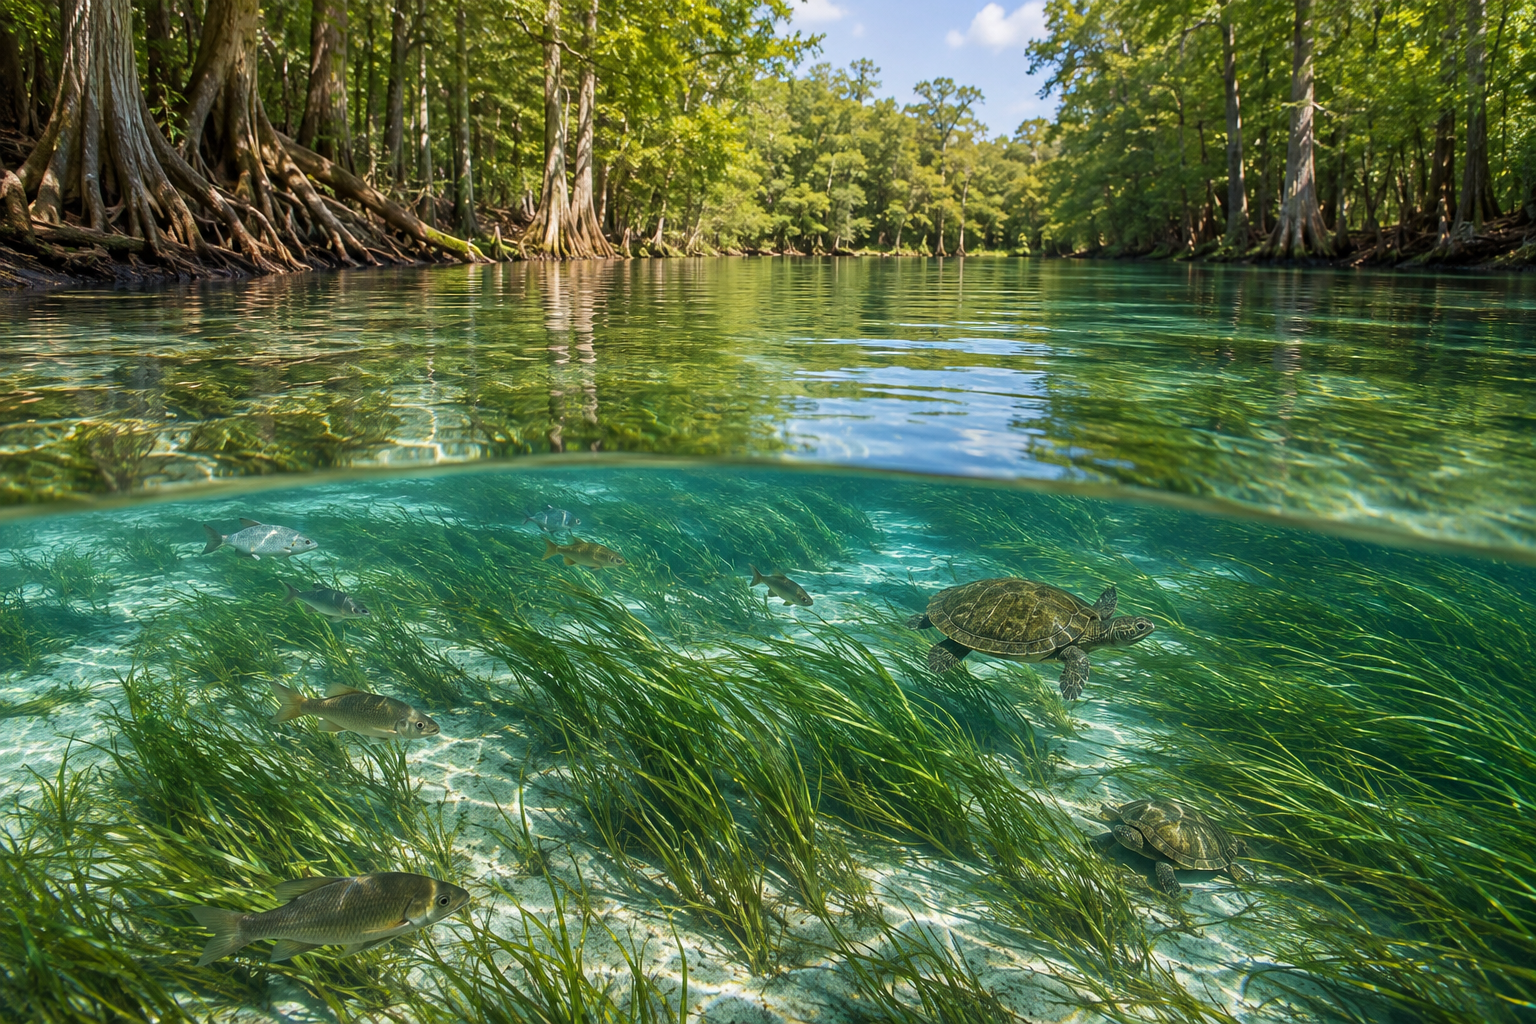
\includegraphics[width=0.6\linewidth]{images/book3/ai/b3-26-clear-spring.png}

{\small Een kalksteenbron: een producentenlaag van zeegras en algen in vol
licht, en daarboven de \omterm{def:b1:ecosystem-organization:trophic}{consumenten} waarvoor de eerste ecologische
energiebalans is opgesteld.}
\end{omfigure}

\section{De stroom van energie}

\begin{definition}[Productiviteit]\label{def:b1:ecosystem-organization:productivity}
\index{primaire productiviteit}\index{bruto primaire productiviteit}\index{netto primaire productiviteit}
De \emph{bruto primaire productiviteit} (BPP) van een \omterm{def:b1:ecosystem-organization:ecosystem}{ecosysteem} is het
tempo waarin zijn \omterm{def:b1:ecosystem-organization:trophic}{producenten} door fotosynthese energie vastleggen, per
eenheid van oppervlak en tijd (\unit{kJ.m^{-2}.yr^{-1}}, of gram koolstof of
droge stof); de \emph{netto primaire productiviteit} (NPP) is wat er na de
eigen ademhaling van de \omterm{def:b1:ecosystem-organization:trophic}{producenten} overblijft --- de organische stof die
werkelijk voor de rest van het systeem beschikbaar komt. \emph{Secundaire
productiviteit} is het tempo waarin \omterm{def:b1:ecosystem-organization:trophic}{consumenten} uit wat zij eten hun eigen
biomassa opbouwen. \emph{Biomassa} is de staande voorraad, de massa die op
een ogenblik aanwezig is; productiviteit is een stroom, biomassa een
voorraad, en de verhouding van de twee is de omzettijd.
\end{definition}

\begin{theorem}[De tienprocentregel]\label{thm:b1:ecosystem-organization:lindeman}
\index{trofische efficiëntie}
Van de energie die als voedsel op één \omterm{def:b1:ecosystem-organization:trophic}{trofisch niveau} binnenkomt bereikt
slechts ongeveer een tiende --- tussen \qty{5}{} en \qty{20}{\%} --- het
volgende niveau als diens voedsel. De rest wordt niet gegeten, wordt niet
opgenomen (vertrekt als ontlasting), of wordt door het niveau zelf verademd.
De beschikbare energie daalt dus tienvoudig per niveau, en daarom overtreffen
\omterm{def:b1:ecosystem-organization:foodweb}{voedselketens} zelden vier of vijf schakels, en zijn de biomassa en de
aantallen van toproofdieren klein.
\end{theorem}
\begin{proof}[Gedeeltelijk bewijs]
De energie die een niveau opneemt is wat het eet min wat het uitscheidt;
daarvan neemt de ademhaling weg wat het niveau aan het leven besteedt
(\cref{ch:b1:organism-environment}), en alleen de rest --- zijn groei en
voortplanting --- is beschikbaar om te worden gegeten. Elk van de drie delen
(gegeten, opgenomen, in biomassa omgezet) ligt ruim onder één: voor een
planteneter op een weide wordt ongeveer \qty{20}{\%} van de plantengroei
gegeten, \qty{50}{\%} daarvan opgenomen en \qty{10}{\%} daarvan in vlees
omgezet, wat \qty{1}{\%} geeft; voor een vleeseter, die meer van zijn prooi
eet en opneemt, ongeveer \qty{10}{\%}. De regel is een waargenomen
regelmaat, geen wet; haar omvang is wat de metingen geven.
\end{proof}
\begin{proof}[Bewijsmateriaal]
Lindeman (1942) mat in een klein meer de energie die het plankton vastlegde
en de energie die op elk niveau daarboven werd vastgehouden en verademd, en
vond dat elk niveau ongeveer een tiende doorgaf. Odum (1957) stelde de
volledige balans van een bron in Florida op: van \qty{1.7e6}{kcal} zonlicht
per vierkante meter per jaar legden de \omterm{def:b1:ecosystem-organization:trophic}{producenten} er \num{20800} vast
(bruto), verademden \num{12000} en lieten \num{8800} netto over; de
planteneters namen \num{3400} en gaven \num{380} aan de vleeseters door; de
vleeseters gaven \num{20} aan de toproofdieren door. De efficiënties waren
\qty{1.2}{\%}, \qty{16}{\%}, \qty{11}{\%} en \qty{5}{\%} --- de
tienprocentregel bij elke stap op een factor twee na.
\end{proof}

\begin{omfigure}
\begin{tikzpicture}[font=\footnotesize, >=Stealth, line cap=round]
  % energy pyramid: widths proportional to log-ish scale of energy
  \fill[omExo!45] (-4.4,0) rectangle (4.4,0.9); \node at (0,0.45) {producenten: netto \num{8800} kcal\,m$^{-2}$\,yr$^{-1}$ (bruto \num{20800})};
  \fill[omProp!45] (-2.9,1.1) rectangle (2.9,2.0); \node at (0,1.55) {planteneters: \num{3400} genomen, \num{1500} opgenomen};
  \fill[omThm!45] (-1.5,2.2) rectangle (1.5,3.1); \node at (0,2.65) {vleeseters: \num{380}};
  \fill[omDef!45] (-0.5,3.3) rectangle (0.5,4.2); \node[anchor=south] at (0,4.25) {toproofdieren: \num{20}};
  \node[anchor=east, align=right] at (-4.6,0.45) {zonlicht:\\ \num{1700000}};
  \node[anchor=east, align=right, gray] at (-3.1,1.55) {\qty{16}{\%}};
  \node[anchor=east, align=right, gray] at (-1.7,2.65) {\qty{11}{\%}};
  \node[anchor=east, align=right, gray] at (-0.7,3.75) {\qty{5}{\%}};
  \draw[->, thick, gray] (4.6,0.45) -- (5.4,0.45) node[right, align=left] {ademhaling en\\ reducenten: warmte};
  \draw[->, thick, gray] (3.1,1.55) -- (5.4,1.55); \draw[->, thick, gray] (1.7,2.65) -- (5.4,2.65); \draw[->, thick, gray] (0.7,3.75) -- (5.4,3.75);
\end{tikzpicture}

{\small De energiebalans van een bron (kilocalorieën per vierkante meter per
jaar). Elk niveau geeft ongeveer een tiende van wat het ontvangt aan het
volgende door; de rest vertrekt als warmte door ademhaling, het meeste ervan
via de \omterm{def:b1:ecosystem-organization:trophic}{reducenten}.}
\end{omfigure}

\begin{proposition}[Piramides]\label{prop:b1:ecosystem-organization:pyramids}
\index{ecologische piramide}
Het stapelen van de \omterm{def:b1:ecosystem-organization:trophic}{trofische niveaus} geeft een \emph{piramide}. Een
piramide van \emph{energie} (de stroom per niveau) staat altijd rechtop: elk
niveau kan alleen minder doorgeven dan het ontving. Een piramide van
\emph{biomassa} (de staande voorraad) staat meestal rechtop maar kan
omgekeerd zijn: op volle zee weegt het fytoplankton, dat zo snel wordt
gegeten als het groeit, op elk ogenblik minder dan het zoöplankton dat ervan
leeft, omdat het in dagen wordt omgezet terwijl de dieren maanden meegaan.
Een piramide van \emph{aantallen} kan elke vorm hebben: één eik voedt
duizenden rupsen. Energie is de eerlijke maat.
\end{proposition}

\begin{method}[Een energiebalans opstellen]\label{met:b1:ecosystem-organization:budget}
\begin{enumerate}
  \item Meet de BPP: met gasuitwisseling (de zuurstof die een perceel of
        een fles in licht en donker afgeeft of de $\mathrm{CO_2}$ die zij
        opneemt: licht min donker geeft bruto, licht alleen geeft netto),
        of door te oogsten (de biomassa die per jaar wordt gewonnen plus
        wat er is gegeten en afgeworpen).
  \item Meet voor elk consumentenniveau de opname (wat het eet), de
        assimilatie (opname min ontlasting), de ademhaling (zijn
        zuurstofverbruik) en de productie (groei plus nakomelingen $=$
        assimilatie min ademhaling).
  \item \omterm{thm:b1:ecosystem-organization:lindeman}{Trofische efficiëntie} tussen niveaus $=$ de productie van het
        bovenste niveau $/$ de productie van het onderste. Ga na dat de
        ademhaling plus de productie plus de afbraak van elk niveau
        optelt tot zijn assimilatie.
  \item Zet alles om in gemeenschappelijke eenheden (\unit{kJ}, of gram
        koolstof bij ongeveer \qty{40}{kJ/g}) en teken de piramide; de som
        van alle ademhaling zou in een \omterm{def:b1:ecosystem-organization:ecosystem}{ecosysteem} in evenwicht over een
        jaar de BPP moeten benaderen.
\end{enumerate}
\end{method}

\begin{example}[Waarom de top dun is]\label{ex:b1:ecosystem-organization:top}
Een vierkante kilometer savanne maakt zo'n \qty{5000}{t} gras per jaar; de
grazers maken er \qty{50}{t} antilope en buffel van; de leeuwen \qty{2}{t}
leeuw --- één of twee dieren. Om een tijger te voeden moet een bos zo groot
zijn dat zijn tiende van een tiende van een tiende van het zonlicht elke week
een heel hert is: honderd vierkante kilometer per tijger, en daarom zijn
grote vleeseters zeldzaam, zwerven zij ver, en verdwijnen zij het eerst
wanneer een \omterm{def:b1:ecosystem-organization:niche}{leefgebied} krimpt.
\end{example}

\begin{proposition}[Productiviteit van de biomen]\label{prop:b1:ecosystem-organization:biomes}
\index{bioom}
De \omterm{def:b1:ecosystem-organization:productivity}{netto primaire productiviteit} per eenheid oppervlak wordt door licht,
temperatuur, water en voedingsstoffen bepaald: tropisch regenwoud
\qtyrange{2000}{3500}{} g droge stof per vierkante meter per jaar; gematigd
bos en bouwland \qtyrange{600}{1500}{}; grasland \qtyrange{200}{1500}{};
toendra en woestijn onder \qty{200}{}; de open oceaan ongeveer \qty{125}{}
(licht in overvloed, voedingsstoffen schaars); opwellingskusten en riffen
\qtyrange{500}{2500}{}. De oceaan, twee derde van de planeet, levert ongeveer
de helft van de wereldproductie; de bossen, een tiende van het land, leveren
een derde van die van het land. Waar water en voedingsstoffen ruim zijn,
volgt de productiviteit licht en warmte; waar zij dat niet zijn, volgt zij
hen.
\end{proposition}

\begin{omfigure}
\begin{tikzpicture}
\begin{axis}[
  xbar, bar width=8pt,
  width=0.84\linewidth, height=6.6cm,
  axis x line=bottom, axis y line=left,
  xmin=0, xmax=2600, xlabel={netto primaire productiviteit (\unit{g.m^{-2}.yr^{-1}}, droge stof)},
  xlabel style={font=\small, at={(axis description cs:0.5,-0.12)}, anchor=north},
  symbolic y coords={woestijn, open oceaan, toendra, gematigd grasland, bouwland, gematigd bos, estuaria en riffen, tropisch regenwoud},
  ytick=data, tick label style={font=\small},
  enlarge y limits=0.08, xtick={0,500,1000,1500,2000,2500},
  nodes near coords, nodes near coords style={font=\scriptsize, anchor=west},
]
\addplot[fill=omExo!45, draw=omExo] coordinates {(90,woestijn) (125,open oceaan) (140,toendra) (600,gematigd grasland) (650,bouwland) (1200,gematigd bos) (1800,estuaria en riffen) (2200,tropisch regenwoud)};
\end{axis}
\end{tikzpicture}

{\small De gemiddelde \omterm{def:b1:ecosystem-organization:productivity}{netto primaire productiviteit} van de belangrijkste
\omterm{prop:b1:ecosystem-organization:biomes}{biomen}. Een twintigvoudig bereik, bepaald door water, warmte, licht en
voedingsstoffen.}
\end{omfigure}

\begin{omfigure}
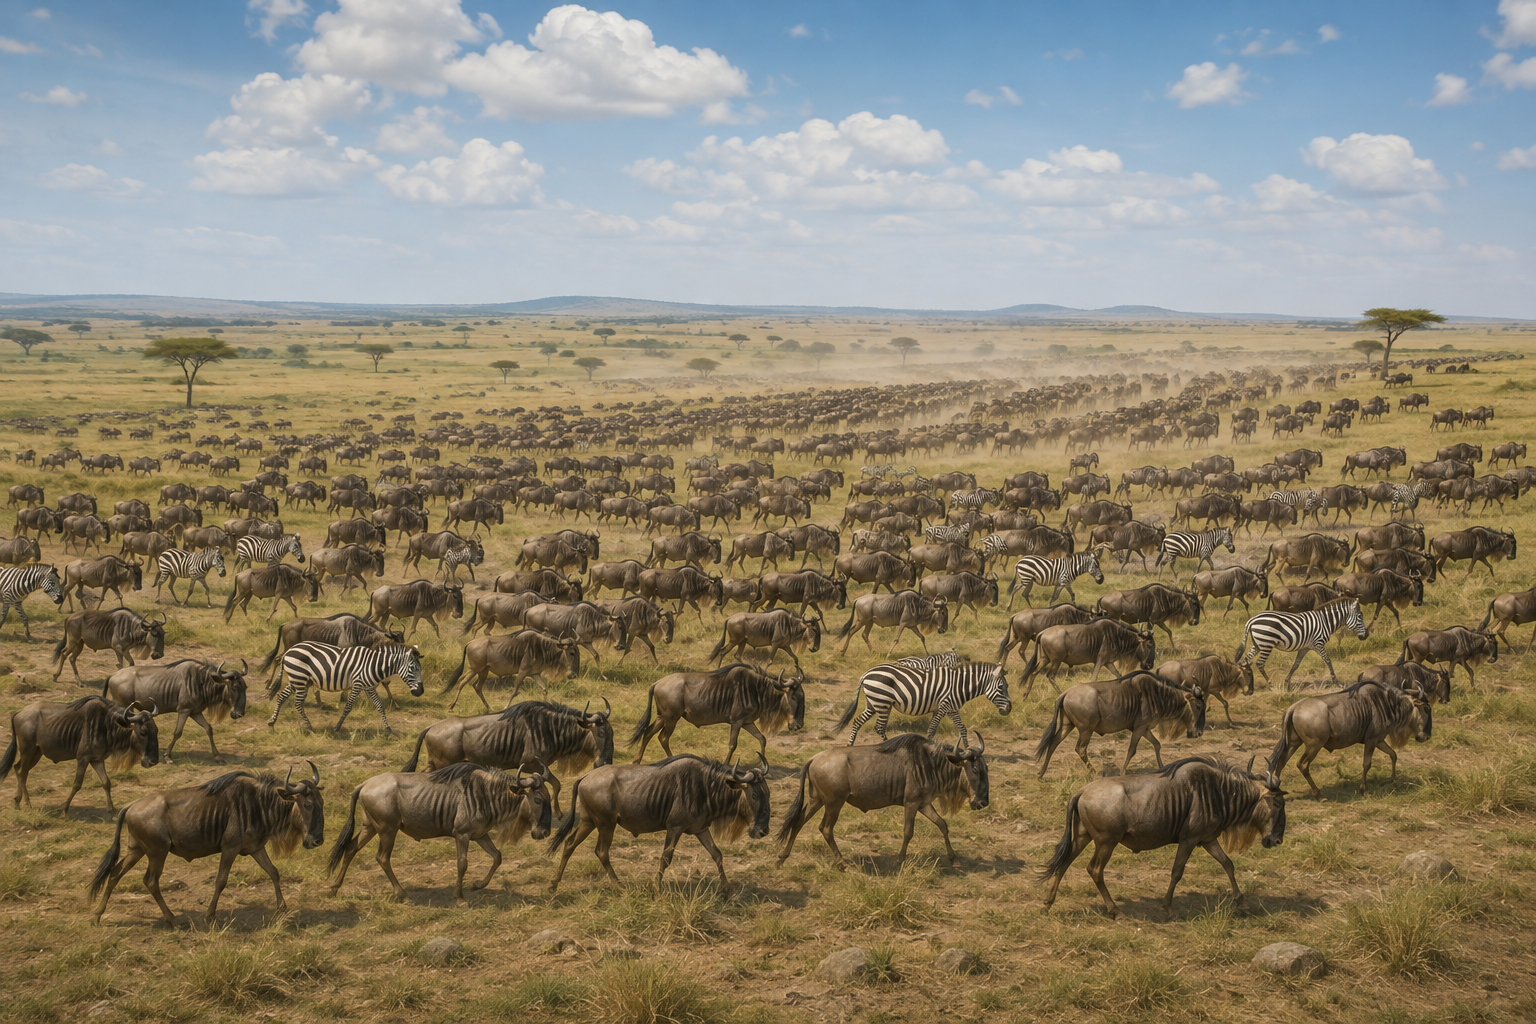
\includegraphics[width=0.6\linewidth]{images/book3/ai/b3-26-wildebeest-migration.png}

{\small Grazers op een savanne: een niveau van primaire \omterm{def:b1:ecosystem-organization:trophic}{consumenten} van een
miljoen dieren, dat de regens volgt die de productiviteit van het gras
bepalen, en een tiende van haar energie naar de roofdieren achter hen draagt.}
\end{omfigure}

\section{Diversiteit tellen}

\begin{definition}[Soortenrijkdom, diversiteitsindex]\label{def:b1:ecosystem-organization:diversity}
\index{soortenrijkdom}\index{shannon-index}
De \emph{soortenrijkdom} $S$ van een \omterm{def:b1:ecosystem-organization:ecosystem}{levensgemeenschap} is het aantal soorten
erin. Rijkdom alleen gaat voorbij aan de talrijkheid: een bos met honderd
eiken en van negen andere bomen elk één is minder divers dan een bos met van
elk tien. De \emph{shannon-index}
\[
H = -\sum_{i=1}^{S} p_i \ln p_i ,
\]
waarin $p_i$ het deel van de individuen is dat tot soort $i$ behoort, stijgt
zowel met de rijkdom als met de \emph{gelijkmatigheid}; hij is $\ln S$
wanneer alle soorten even talrijk zijn en bijna nul wanneer er één
overheerst. De \emph{gelijkmatigheid} is $H/\ln S$. De diversiteit stijgt in
het algemeen van de polen naar de tropen, met het oppervlak, met de tijd
sinds de laatste verstoring, en tot op zekere hoogte met de productiviteit
van de plek.
\end{definition}

\begin{method}[Een levensgemeenschap bemonsteren]\label{met:b1:ecosystem-organization:sampling}
\begin{enumerate}
  \item Bemonster met een methode die bij de \omterm{def:b1:organism-environment:organism}{organismen} past
        (proefvlakken, netten, vallen, transecten) en noteer het aantal
        individuen van elke soort.
  \item Zet het aantal gevonden soorten uit tegen het aantal monsters (of
        individuen): de kromme stijgt steil en vlakt dan af; waar zij
        afvlakt is de rijkdom vrijwel volledig. Vergelijk
        \omterm{def:b1:ecosystem-organization:ecosystem}{levensgemeenschappen} alleen bij een gelijke bemonsteringsinspanning.
  \item Bereken $H$ en de gelijkmatigheid; vergelijk die met de
        rang--talrijkheidsgrafiek (soorten naar talrijkheid gerangschikt,
        op een logaritmische schaal), waarvan de helling de overheersing
        toont.
  \item Duid het: een lage gelijkmatigheid wijst op een overheersende soort
        of op stress; een daling van $H$ in de tijd wijst op een
        verandering in de \omterm{def:b1:ecosystem-organization:ecosystem}{biotoop}.
\end{enumerate}
\end{method}

\begin{example}[Twee bossen]\label{ex:b1:ecosystem-organization:twowoods}
Bos A: 100 eiken en van negen andere bomen elk één; $H = -(0.917\ln
0.917 + 9\times 0.0092\ln 0.0092) = 0.08 + 0.39 = 0.47$, gelijkmatigheid
$0.47/2.30 = 0.20$. Bos B: van dezelfde tien soorten elk tien; $H =
\ln 10 = 2.30$, gelijkmatigheid 1. Dezelfde rijkdom, vijf keer de
diversiteit.
\end{example}

\section{Opgaven}

\begin{exercise}[$\star$]\label{exo:b1:ecosystem-organization:1}
Omschrijf \omterm{def:b1:ecosystem-organization:ecosystem}{ecosysteem}, \omterm{def:b1:ecosystem-organization:ecosystem}{levensgemeenschap} en \omterm{def:b1:ecosystem-organization:ecosystem}{biotoop}, met een vijver als voorbeeld.
\end{exercise}

\begin{exercise}[$\star$]\label{exo:b1:ecosystem-organization:2}
Onderscheid \omterm{def:b1:ecosystem-organization:niche}{leefgebied} van \omterm{def:b1:ecosystem-organization:niche}{nis}, en fundamentele van gerealiseerde \omterm{def:b1:ecosystem-organization:niche}{nis}.
\end{exercise}

\begin{exercise}[$\star$]\label{exo:b1:ecosystem-organization:3}
Bereken uit de energiepiramide van de bron de efficiëntie van zonlicht naar
bruto productie, en het deel van de netto productie dat de planteneters
namen.
\end{exercise}

\begin{exercise}[$\star$]\label{exo:b1:ecosystem-organization:4}
Noem de vier trofische groepen en zeg welke de kringloop van de stof sluit.
\end{exercise}

\begin{exercise}[$\star\star$]\label{exo:b1:ecosystem-organization:5}
De NPP van een weide is \qty{800}{g.m^{-2}.yr^{-1}} (\qty{17}{kJ/g}).
Konijnen eten er \qty{15}{\%} van, nemen \qty{50}{\%} van wat zij eten op,
en zetten \qty{5}{\%} van wat zij opnemen om in konijn. Bereken de
konijnenproductie per hectare en de \omterm{thm:b1:ecosystem-organization:lindeman}{trofische efficiëntie} van NPP naar
konijn.
\end{exercise}

\begin{exercise}[$\star\star$]\label{exo:b1:ecosystem-organization:6}
Leg uit waarom een piramide van biomassa in zee omgekeerd kan zijn maar een
piramide van energie nooit.
\end{exercise}

\begin{exercise}[$\star\star$]\label{exo:b1:ecosystem-organization:7}
Bereken de \omterm{def:b1:ecosystem-organization:diversity}{shannon-index} en de gelijkmatigheid voor een monster van 50 A,
30 B, 15 C en 5 D. Vergelijk dat met vier soorten van elk 25.
\end{exercise}

\begin{exercise}[$\star\star$]\label{exo:b1:ecosystem-organization:8}
In een proef met een lichte en een donkere fles stijgt de zuurstof in de
lichte fles op één dag met \qty{3}{mg/L} en daalt zij in de donkere met
\qty{1}{mg/L}. Bereken de bruto en de netto productiviteit van het water in
milligram zuurstof per liter per dag, en in gram koolstof (\qty{1}{g}
$\mathrm{O_2}$ $\approx$ \qty{0.375}{g} C).
\end{exercise}

\begin{exercise}[$\star\star$]\label{exo:b1:ecosystem-organization:9}
Waarom bestaan er geen \omterm{def:b1:ecosystem-organization:foodweb}{voedselketens} van tien schakels, en waarom hebben
eilanden en woestijnen kortere ketens dan bossen?
\end{exercise}

\begin{exercise}[$\star\star\star$]\label{exo:b1:ecosystem-organization:10}
Een mens kan graan rechtstreeks eten of het aan runderen voeren. Bereken bij
een \omterm{thm:b1:ecosystem-organization:lindeman}{trofische efficiëntie} van \qty{10}{\%} voor runderen het land dat nodig
is om één persoon met rundvlees te voeden tegenover met graan, als de akker
\qty{6}{t} graan per hectare geeft en een persoon \qty{1}{t} per jaar nodig
heeft. Wat zegt dat over het trofische niveau van de mens en over de
draagkracht van de planeet?
\end{exercise}

\begin{exercise}[$\star\star\star$]\label{exo:b1:ecosystem-organization:11}
De open oceaan heeft een lage NPP per vierkante meter maar de helft van de
wereldproductie. Breng die twee met elkaar in overeenstemming, en leg uit
waarom de visserij op zee zich in enkele procenten van haar oppervlak
concentreert.
\end{exercise}

\begin{exercise}[$\star\star\star$]\label{exo:b1:ecosystem-organization:12}
``Een \omterm{def:b1:ecosystem-organization:ecosystem}{ecosysteem} is een machine die zonlicht in warmte omzet, met het leven
als bijproduct.'' Bespreek dat in een alinea: de energiestroom tegenover de
kringloop van de stof, wat de \omterm{def:b1:ecosystem-organization:trophic}{reducenten} doen, en wat de zin weglaat.
\end{exercise}

\section{Vraagstuk: de balans van een bron}

\begin{problem}[{Weekendvraagstuk --- de bron van Odum niveau voor niveau
opgesteld: zonlicht naar gras, gras naar slak, slak naar vis, vis naar
reiger, met de ademhaling en de reducenten, eindigend op de trofische
efficiënties bij elk niveau}]
\label{pb:b1:ecosystem-organization:1}
Een bron ontvangt \qty{1.7e6}{kcal} zonlicht per vierkante meter per jaar.
Haar \omterm{def:b1:ecosystem-organization:trophic}{producenten} leggen \qty{20800}{kcal} vast (bruto) en verademen
\qty{12000}{}. Planteneters eten \qty{3400}{kcal} plantenstof, waarvan zij
\qty{1500}{} opnemen, \qty{1100}{} verademen en de rest in groei en
nakomelingen omzetten. Vleeseters eten \qty{380}{kcal}, verademen
\qty{300}{} en produceren de rest; toproofdieren eten \qty{20}{kcal},
verademen \qty{14}{} en produceren \qty{6}{}. Alles wat niet wordt gegeten
of verademd gaat naar de \omterm{def:b1:ecosystem-organization:trophic}{reducenten}, die het verademen. Neem
\qty{1}{kcal} $= \qty{4.18}{kJ}$ en \qty{10}{kcal} per gram droge biomassa.

\medskip
\noindent\textbf{Deel I --- De \omterm{def:b1:ecosystem-organization:trophic}{producenten}.}
\begin{enumerate}
  \item Bereken de \omterm{def:b1:ecosystem-organization:productivity}{netto primaire productiviteit}.
  \item Bereken het rendement van de fotosynthese: de bruto productie
        gedeeld door het zonlicht. Vergelijk dat met de \qty{34}{\%} van
        \cref{ch:b1:photosynthesis} en noem drie verliezen die de twee
        scheiden.
  \item Welk deel van de bruto productie verademen de \omterm{def:b1:ecosystem-organization:trophic}{producenten}?
  \item Hoeveel van de netto productie wordt door planteneters gegeten,
        en hoeveel gaat rechtstreeks naar de \omterm{def:b1:ecosystem-organization:trophic}{reducenten}?
  \item Druk de NPP uit in gram droge stof per vierkante meter per jaar
        en plaats de bron tussen de \omterm{prop:b1:ecosystem-organization:biomes}{biomen} van het hoofdstuk.
  \item Hoeveel van het zonlicht verlaat de bron per vierkante meter en
        per jaar als warmte zonder ooit door een levend \omterm{def:b1:organism-environment:organism}{organisme} te zijn
        gegaan?
\end{enumerate}

\medskip
\noindent\textbf{Deel II --- De \omterm{def:b1:ecosystem-organization:trophic}{consumenten}.}
\begin{enumerate}[resume]
  \item Bereken de productie van de planteneters en hun
        assimilatierendement (opgenomen/gegeten).
  \item Bereken het productierendement van de planteneters
        (productie/opgenomen).
  \item Bereken de \omterm{thm:b1:ecosystem-organization:lindeman}{trofische efficiëntie} van \omterm{def:b1:ecosystem-organization:trophic}{producenten} naar
        planteneters: de productie van de planteneters gedeeld door de
        netto primaire productie.
  \item Bereken de productie van de vleeseters en de \omterm{thm:b1:ecosystem-organization:lindeman}{trofische
        efficiëntie} van planteneters naar vleeseters.
  \item Bereken de \omterm{thm:b1:ecosystem-organization:lindeman}{trofische efficiëntie} van vleeseters naar
        toproofdieren.
  \item Hoeveel energie per vierkante meter per jaar bereikt het eigen
        \omterm{def:b1:body-plans-tissues:tissue}{weefsel} van het toproofdier? Welk deel van het zonlicht is dat?
  \item Waarom stijgt het assimilatierendement van planteneters naar
        vleeseters?
\end{enumerate}

\medskip
\noindent\textbf{Deel III --- De \omterm{def:b1:ecosystem-organization:trophic}{reducenten} en de balans.}
\begin{enumerate}[resume]
  \item Noem elke stroom naar de \omterm{def:b1:ecosystem-organization:trophic}{reducenten} (niet gegeten netto productie,
        ontlasting van de planteneters en niet gegeten productie van de
        planteneters, enzovoort) en tel ze op.
  \item Bereken de totale ademhaling van het \omterm{def:b1:ecosystem-organization:ecosystem}{ecosysteem}: \omterm{def:b1:ecosystem-organization:trophic}{producenten},
        planteneters, vleeseters, toproofdieren en \omterm{def:b1:ecosystem-organization:trophic}{reducenten}.
  \item Vergelijk die met de bruto productie. Wat betekent de
        vergelijking voor de biomassa van de bron over een jaar?
  \item Welk deel van de bruto productie wordt door de \omterm{def:b1:ecosystem-organization:trophic}{reducenten}
        verademd?
  \item Teken de energiepiramide met de productie van de vier niveaus en
        zet de efficiënties erbij.
\end{enumerate}

\medskip
\noindent\textbf{Deel IV --- Voorraden, omzet en verandering.}
De staande biomassa is \qty{800}{g/m^2} \omterm{def:b1:ecosystem-organization:trophic}{producenten}, \qty{40}{g/m^2}
planteneters, \qty{10}{g/m^2} vleeseters en \qty{1.5}{g/m^2}
toproofdieren.
\begin{enumerate}[resume]
  \item Zet elke biomassa om in kilocalorieën en teken de piramide van de
        biomassa. Staat zij rechtop?
  \item Bereken de omzettijd (biomassa/productie) van elk niveau. Welk
        niveau wordt het snelst omgezet, en waarom?
  \item Een reiger van \qty{2}{kg} leeft van de productie van de
        toproofdieren van de bron. Hoeveel vierkante meter heeft hij
        nodig?
  \item De bron wordt met meststof verrijkt en haar bruto productie
        verdubbelt, maar de planteneters kunnen niet sneller eten. Wat
        gebeurt er met de extra productie, met de ademhaling van de
        \omterm{def:b1:ecosystem-organization:trophic}{reducenten}, en met de zuurstof van het water 's nachts?
  \item Er wordt een nieuwe vis uitgezet die de eieren van de planteneters
        eet en hun productie halveert. Voorspel de productie van de
        vleeseters en het aantal reigers, en het lot van het zeegras.
  \item Leg uit waarom het wegnemen van de toproofdieren het zeegras veel
        sterker zou veranderen dan het wegnemen van evenveel energie aan
        planteneters.
  \item Geef het resultaat: de \omterm{thm:b1:ecosystem-organization:lindeman}{trofische efficiënties} bij elk van de drie
        overdrachten, het rendement van zonlicht naar bruto productie, en
        het deel van de zonne-energie dat de toproofdieren bereikt.
\end{enumerate}
\end{problem}
